\documentclass{article}

\usepackage[T1, T2A]{fontenc}
\usepackage[utf8x]{inputenc}
\usepackage[russianb]{babel}
\usepackage{vmargin}
\usepackage{amsmath}
\usepackage{amsfonts}
\usepackage{halloweenmath}
\usepackage{amssymb}
\usepackage{cancel}
\usepackage{mathrsfs}
\usepackage{cancel}

\usepackage{graphicx}
\graphicspath{https://github.com/IlidanNaga/317_Hometask_Practicum/tree/master/Big_task_1/Images}
\usepackage{wrapfig}

\title{KNNClassifier report}
\author{Kornilov Maxim, group 317}
\date{October 2019}

\begin{document}

\maketitle

\textbf{\Large План отчета:}

\begin{enumerate}
    \item \text{Список файлов проекта} 
    \item \text{Эксперимент 1} 
    \item \text{Эксперимент 2} 
    \item \text{Эксперимент 3} 
    \item \text{Эксперимент 4} 
    \item \text{Типовые и шумовые ошибки} 
    \item \text{Применение rotate} 
    \item \text{Применение gaussian filter} 
    \item \text{Применение shift} 
    \item \text{Применение rotate + gaussian filter} 
    \item \text{Применение всех методов}
    \item \text{Вывод}
\end{enumerate}

\textbf{\Large Список файлов проекта:} \\
\begin{verbatim}
    nearest_neighbors.py - модуль с реализацией классификатора 
    cross_validation.py - модуль с реализацией кросс-валидации 
    distances.py - модуль метрик
\end{verbatim} \\

\textbf{\large Для всех экспериментов, где не оговорено иное, применялась случайная подвыборка датасета из 3500 объектов, которая разбивалась на 3 фолда} \\

% Начало блока Эксперимент 1
\textbf{\Large Эксперимент 1:} \\
\begin{verbatim}
Файл: completing_task_1.py
\end{verbatim}
Цель эксперимента - проверить качество работы классификатора на подвыборке признаков различных размеров, затем - сравнить работу различных методов классификации \\
Подвыборка признаков получалась случайным образом посредством shuffle \\

\begin{verbatim}
Пример вывода программы, для большего понимания:
    Accuracy for: 
    10 - 0.19799999999999995
    20 - 0.46799999999999997
    100 - 0.836
    200 - 0.888
    my_own: accuracy = 0.924, time = 48.8452889919281
    my cosine: accuracy = 0.94, time = 0.10344433784484863
    my weight euc: accuracy = 0.928, time = 38.494842290878296
    my weight cos: accuracy = 0.944, time = 0.1073000431060791
    kd_tree: accuracy = 0.924, time = 0.4562821388244629
    kd_weight: accuracy = 0.928, time = 0.37099337577819824
    brute: accuracy = 0.924, time = 0.14404988288879395
    brute_weight: accuracy = 0.928, time = 0.13192200660705566
    ball_tree: accuracy = 0.924, time = 0.2951321601867676
    ball_weight: accuracy = 0.928, time = 0.27849483489990234
\end{verbatim}
 
\textit{\large Число признаков:} \\
10 - Точность в таком случае может быть от 0.15 до 0.5 \\
20 - Точность в таком случае может быть от 0.3 до 0.6 \\
100 - Точность в таком случае может быть от 0.8 до 0.85 \\
200 - Точность в таком случае может быть от 0.85 до 0.9 \\
Для сравнения, точность при всех признаках варьируется от 0.9 до 0.925
Итог: При повышении числа признаков значимым будет только повышение до ~100 признаков, по ходу которого будет значительный прирост точности, большее число признаков может быть откинуто для ускорения рассчётов без значительных потерь в точности (но, всё равно, нежелательно) \\

\textit{\large Зависимость точности от метода:}
\begin{itemize}
    \item В силу построения методов, различий между ними может быть 3:\begin{itemize}
        \item cosine или euclidean метрика, влияет на точность и время работы алгоритма
        \item метод нахождения ближайших соседей, влияет на время работы алгоритма
        \item используются ли веса при рассчетах, влияет на точность и время работы алгоритма
    \end{itemize}
    \item Точность: \begin{itemize}
        \item Методы с cosine метрикой показывают более высокую точность относительно аналогичных с euclidean метрикой
        \item Методы с весами всегда (euclidean) или почти всегда (cosine) показывают более высокую точность относительно аналогичных без весов
        \item Самую высокую точность показали: brute + cosine + weights и my own + cosine + weights
    \end{itemize}
    \item Время работы: \begin{itemize}
        \item Методы, реализованные в sklearn.neighbors.KNeighborsClassifier имеют примерно одинаковое время работы
        \item Самый медленный метод - my own + euclidean, с весами или нет
        \item Самый быстрый метод - my own + cosine
    \end{itemize}
\end{itemize}

\textit{\large\textbf{Вывод: }Оптимальным будет метод с косинусной метрикой и весами} \\

% Начало блока Эксперимент 2
\textbf{\Large Эксперимент 2:}  \\
\begin{verbatim}
    Файл: completing_task_2.py
\end{verbatim}
Цель эксперимента - найти количество с, оптимальное для классификации на оптимальном методе

\texit{Ход эксперимента: } - берём метод, который лучше всего себя проявил на прошлом эксперименте (в качестве сравнения с ним так же возьмём brute + euclidean, т.к. он работает аналогично my own + euclidean, но быстрее), а именно - my own + cosine и проведём на подвыборке кросс-валидацию с 3 фолдами и k от 1 до 10

Результат: Лучшую точность алгоритм показал на k = 4 \\

% Начало блока Эксперимент 3
\textbf{\Large Эксперимент 3:} \\
\begin{verbatim}
    Файл: completing_task_3.py
\end{verbatim}
Цель эксперимента - определить, какой метод покажет более высокую точность - взвешенный или нет, определить максимальную точность в зависимости от наличия весов и количества соседей

\textit{Ход эксперимента: } запускаем кросс-валидацию с 3 фолдами и k от 1 до 10 на лучшем из методов - my own + cosine с весами и без них, и определяем оптимальные параметры

\textit{Вывод: } Оптимальный метод - my own + cosine + weights, k = 4 \\

% Начало блока Эксперимент 4
\textbf{\Large Эксперимент 4:} \\
\begin{verbatim}
    Файл: completing_task_4.py
\end{verbatim}
Цель эксперимента - получить результат работы всего датасета на оптимальном методе.

\textit{Ход эксперимента: }\begin{itemize}
    \item Разобьём датасет на 2 части, размером 60k и 10k, случайным образом с random state=666 (для того, чтобы не передавать тестовую подвыборку в другие файлы и не перерассчитывать knn каждый раз)
    \item Обучим и проверим KNNClassifier с параметрами strategy = my own, metric = cosine, weight = True, test block size = 0
    \item Сохраним предсказанные классы для дальнейшей визуализации
\end{itemize}

\textit{Результат: } accuracy = 0.9756 \\

% Начало нового блока 
\textbf{\Large Типовые и шумовые ошибки:} \\
\begin{verbatim}
    Файл: confusion_matrix_build.ipynb
\end{verbatim}
Цель эксперимента - посмотреть, что из себя представляют ошибки нашего алгоритма, охарактеризовать их

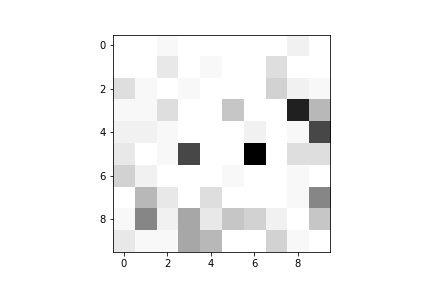
\includegraphics{error_map}

\textbf{\Large Применение метода rotate:} \\

\textbf{\Large Применение метода gaussian filter:} \\

\textbf{\Large Применение метода сдвига:} \\

\textbf{\Large Применение комбинации методов: gaussian filter + rotate:} \\

\textbf{\Large Применение комбинации 3 методов:} \\

\textbf{\Large Вывод:}

\end{document}
